%%%%%%%%%%%%%%%%%%%%%%%%%%%%%%%%%%%%%%%%%
% Arsclassica Article
% LaTeX Template
% Version 1.1 (1/8/17)
%
% This template has been downloaded from:
% http://www.LaTeXTemplates.com
%
% Original author:
% Lorenzo Pantieri (http://www.lorenzopantieri.net) with extensive modifications by:
% Vel (vel@latextemplates.com)
%
% License:
% CC BY-NC-SA 3.0 (http://creativecommons.org/licenses/by-nc-sa/3.0/)
%
%%%%%%%%%%%%%%%%%%%%%%%%%%%%%%%%%%%%%%%%%

%----------------------------------------------------------------------------------------
%	PACKAGES AND OTHER DOCUMENT CONFIGURATIONS
%----------------------------------------------------------------------------------------

\documentclass[
10pt, % Main document font size
a4paper, % Paper type, use 'letterpaper' for US Letter paper
oneside, % One page layout (no page indentation)
%twoside, % Two page layout (page indentation for binding and different headers)
headinclude,footinclude, % Extra spacing for the header and footer
BCOR5mm, % Binding correction
]{scrartcl}

%%%%%%%%%%%%%%%%%%%%%%%%%%%%%%%%%%%%%%%%%
% Arsclassica Article
% Structure Specification File
%
% This file has been downloaded from:
% http://www.LaTeXTemplates.com
%
% Original author:
% Lorenzo Pantieri (http://www.lorenzopantieri.net) with extensive modifications by:
% Vel (vel@latextemplates.com)
%
% License:
% CC BY-NC-SA 3.0 (http://creativecommons.org/licenses/by-nc-sa/3.0/)
%
%%%%%%%%%%%%%%%%%%%%%%%%%%%%%%%%%%%%%%%%%

%----------------------------------------------------------------------------------------
%	REQUIRED PACKAGES
%----------------------------------------------------------------------------------------

\usepackage[
nochapters, % Turn off chapters since this is an article        
beramono, % Use the Bera Mono font for monospaced text (\texttt)
eulermath,% Use the Euler font for mathematics
pdfspacing, % Makes use of pdftex’ letter spacing capabilities via the microtype package
dottedtoc % Dotted lines leading to the page numbers in the table of contents
]{classicthesis} % The layout is based on the Classic Thesis style

\usepackage{arsclassica} % Modifies the Classic Thesis package

\usepackage[T1]{fontenc} % Use 8-bit encoding that has 256 glyphs

\usepackage[utf8]{inputenc} % Required for including letters with accents

\usepackage{graphicx} % Required for including images
\graphicspath{{Figures/}} % Set the default folder for images

\usepackage{enumitem} % Required for manipulating the whitespace between and within lists

\usepackage{lipsum} % Used for inserting dummy 'Lorem ipsum' text into the template

\usepackage{subfig} % Required for creating figures with multiple parts (subfigures)

\usepackage{amsmath,amssymb,amsthm} % For including math equations, theorems, symbols, etc

\usepackage{varioref} % More descriptive referencing

%----------------------------------------------------------------------------------------
%	THEOREM STYLES
%---------------------------------------------------------------------------------------

\theoremstyle{definition} % Define theorem styles here based on the definition style (used for definitions and examples)
\newtheorem{definition}{Definition}

\theoremstyle{plain} % Define theorem styles here based on the plain style (used for theorems, lemmas, propositions)
\newtheorem{theorem}{Theorem}

\theoremstyle{remark} % Define theorem styles here based on the remark style (used for remarks and notes)

%----------------------------------------------------------------------------------------
%	HYPERLINKS
%---------------------------------------------------------------------------------------

\hypersetup{
%draft, % Uncomment to remove all links (useful for printing in black and white)
colorlinks=true, breaklinks=true, bookmarks=true,bookmarksnumbered,
urlcolor=webbrown, linkcolor=RoyalBlue, citecolor=webgreen, % Link colors
pdftitle={}, % PDF title
pdfauthor={\textcopyright}, % PDF Author
pdfsubject={}, % PDF Subject
pdfkeywords={}, % PDF Keywords
pdfcreator={pdfLaTeX}, % PDF Creator
pdfproducer={LaTeX with hyperref and ClassicThesis} % PDF producer
} % Include the structure.tex file which specified the document structure and layout

\hyphenation{Fortran hy-phen-ation} % Specify custom hyphenation points in words with dashes where you would like hyphenation to occur, or alternatively, don't put any dashes in a word to stop hyphenation altogether

%----------------------------------------------------------------------------------------
%	TITLE AND AUTHOR(S)
%----------------------------------------------------------------------------------------

\title{\normalfont\spacedallcaps{DAA}} % The article title

%\subtitle{Subtitle} % Uncomment to display a subtitle

\author{\spacedlowsmallcaps{José Luis Leiva Fleitas- 412* \& Eduardo García Maleta-411\textsuperscript{1}}} % The article author(s) - author affiliations need to be specified in the AUTHOR AFFILIATIONS block

\date{} % An optional date to appear under the author(s)

%----------------------------------------------------------------------------------------

\begin{document}

%----------------------------------------------------------------------------------------
%	HEADERS
%----------------------------------------------------------------------------------------

\renewcommand{\sectionmark}[1]{\markright{\spacedlowsmallcaps{#1}}} % The header for all pages (oneside) or for even pages (twoside)
%\renewcommand{\subsectionmark}[1]{\markright{\thesubsection~#1}} % Uncomment when using the twoside option - this modifies the header on odd pages
\lehead{\mbox{\llap{\small\thepage\kern1em\color{halfgray} \vline}\color{halfgray}\hspace{0.5em}\rightmark\hfil}} % The header style

\pagestyle{scrheadings} % Enable the headers specified in this block

%----------------------------------------------------------------------------------------
%	TABLE OF CONTENTS & LISTS OF FIGURES AND TABLES
%----------------------------------------------------------------------------------------

\maketitle % Print the title/author/date block

\setcounter{tocdepth}{2} % Set the depth of the table of contents to show sections and subsections only

\tableofcontents % Print the table of contents

\listoffigures % Print the list of figures

\listoftables % Print the list of tables

%----------------------------------------------------------------------------------------
%	ABSTRACT
%----------------------------------------------------------------------------------------

\section*{Abstract} % This section will not appear in the table of contents due to the star (\section*)

\lipsum[1] % Dummy text

%----------------------------------------------------------------------------------------
%	AUTHOR AFFILIATIONS
%----------------------------------------------------------------------------------------

\let\thefootnote\relax\footnotetext{* \textit{Department of Biology, University of Examples, London, United Kingdom}}

\let\thefootnote\relax\footnotetext{\textsuperscript{1} \textit{Department of Chemistry, University of Examples, London, United Kingdom}}

%----------------------------------------------------------------------------------------

\newpage % Start the article content on the second page, remove this if you have a longer abstract that goes onto the second page

%----------------------------------------------------------------------------------------
%	Corrupcion
%----------------------------------------------------------------------------------------

\section{Corrupción}

Problema: \\

Han pasado 20 años desde que Lidier se graduó de Ciencias de la Computación  
(haciendo una muy buena tesis) y las vueltas de la vida lo llevaron a convertirse  
en el presidente del Partido Comunista de Cuba. Una de sus muchas responsabilidades  
consiste en visitar zonas remotas. En esta ocasión debe visitar una  
ciudad campestre de Pinar del Río.\\

También han pasado 20 años desde que Marié consiguió su título en MATCOM.  
Tras años de viaje por las grandes metrópolis del mundo, en algún punto  
decidió que prefería vivir una vida tranquila, aislada de la urbanización, en una  
tranquila ciudad de Pinar del Río. Las vueltas de la vida quisieron que precisamente  
Marié fuera la única universitaria habitando la ciudad que Lidier se  
dispone a visitar.\\

Los habitantes de la zona entraron en pánico ante la visita de una figura tan  
importante y decidieron reparar las calles de la ciudad por las que transitaría  
Lidier. El problema está en que nadie sabía qué ruta tomaría el presidente y  
decidieron pedirle ayuda a Marié.

La ciudad tiene $n$ puntos importantes, unidos entre sí por calles cuyos  
tamaños se conoce. Se sabe que Lidier comenzará en alguno de esos puntos  
($s$) y terminará el viaje en otro ($t$). Los ciudadanos quieren saber, para  
cada par $s$, $t$, cuántas calles participan en algún camino de distancia mínima  
entre $s$ y $t$. \\

\subsection{Modelacion del problema}

Representaremos la ciudad como un grafo dirigido $G = {V,E}$, donde los $n$ puntos importantes
de la ciudad estarán representados por $n$ vértices $(V)$ del grafo $G$ y las calles que unen estos 
puntos estarán representadas por las aristas de dicho grafo $(E)$. Entonces el problema lo analizaremos
de la siguiente manera:

Sea $G = {V,E}$ un grafo,se quiere, para todo par de vértices $s$ y $t$ del grafo, determinar cuántas aristas 
participan en algún camino de distancia mínima entre $s$ y $t$.


\subsection{Solución 1: Utilizando el algoritmo de Dijkstra}

Se le realiza la siguiente modificación al algoritmo de Dijkstra : se le 
añade un diccionario $caminos$ cuyas llaves son los vértices del grafo 
y el valor de cada llave será el padre de cada vértice en el camino de distancia 
mínima entre el vértice de inicio y él. Mediante este diccionario podremos reconstruir 
luego los caminos de distancia mínima entre el vértice de inicio y los restantes. \\

Tenemos la función $reconstruir_camino$ que se encarga de devolver el camino entre 2 vértices. Esto 
lo utilizamos en nuestro algoritmo ya sabiendo que el camino entre estos des vértices es un camino de 
distancia mínima.\\

Luego, para darle solución al problema, tenemos la función $solver$ que calcula la cardinalidad de algún 
camino de distancia mínima entre todos los pares de vértices del grafo.

\subsection{Análisis de Correctitud}

La función $solver$ se basa en el algoritmo de Dikstra para calcular las distancias mínimas desde 
cada vértice a todos los demás vértices en el grafo. A continuación se desglosan los pasos que se realizan:\\

- Inicialización :\\
Se crea un diccionario ${long_de_caminos}$ que almacenará la longitud de los caminos mínimos entre cada par de 
vértices.


- Iteración sobre cada vértice :\\ 
Para cada vértice $v$ del grafo, se ejecuta el algoritmo de Dijkstra, obteniendo las distancias y los caminos desde $v$
a todos los demás vértices.

Uso del diccionario de $caminos$. Este se utiliza para rastrear el camino más corto desde el vértice inicial hasta cada 
vértice en el grafo. Cada vez que se realiza una operación de relajación en el algoritmo, se actualiza el padre del vértice 
que está siendo relajado. Esto asegura que, al final del algoritmo, podemos reconstruir el camino más corto desde el vértice inicial
hasta cualquier otro vértice utilizando este diccionario.


- Reconstrucción del camino : \\
Para cada par de vértices $v$ y $w$, si estos son distintos, se reconstruye el camino mínimo utilizando la función $reconstruir_camino$. Luego, 
si existe un camino, se almacenará la longitud de este en el diccionario\\


Correctitud : \\
El algoritmo de Dijkstra garantiza que las distancias calculadas son las mínimas desde el vértice inicial $v$. Por lo tanto, 
cualquier camino reconstruido utilizando esas distancias es correcto. Luego, después de reconstruir los caminos con la función $reconstruir_camino$, 
lo que se almacena en el diccionario $long_de_caminos$ son las longitudes de los caminos de distancia minima entre todo par de 
vértices.


\subsection{Análisis de Complejidad Temporal}

1. Complejidad de Dijkstra:\\

La complejidad temporal del algoritmo Dijkstra utilizando una cola de prioridad (heap) es $O((V+E)log(V))$, donde $V$ es el número de vértices y $E$ es el número de 
aristas en el grafo.\\

2. Llamadas a Dijkstra:\\

En nuestra función $Solver$, se llama a Dijkstra desde cada vértice, lo que implica que se sejecuta $V$ veces. 
Por lo tanto, la complejidad total por esta parte es $O(V*(V+E)log(V))$. \\

3. Reconstrucción del camino:\\

La reconstrucción del camino tiene una complejidad lineal en función del número de vértices en el camino, que en el peor 
de los casos es $O(V)$. Sin embargo, esta función se llama para cada par de vértices, lo que significa que se invoca una vez por cada 
combinación de vértices diferentes (v,w). Por tanto, son un toal de $V*(V-1)$ invocaiones. Esto implica que la complejidad total derivada de la 
reconstrucción es $O(V^3)$. \\

Sumando todo, la complejidad total del algoritmo $solver$ es: $O(V^2 * log(V) + V * E*log(V) ) + O(V^3)$. \\

En un grafo denso donde $E$ puede ser aproximadamente $V^2$, el caso peor sería $O(V^3)$





A statement requiring citation \cite{Figueredo:2009dg}.


 
%----------------------------------------------------------------------------------------
%	METHODS
%----------------------------------------------------------------------------------------

\section{Banco}

Eduardo es el gerente principal de un gran banco. Tiene acceso ilimitado al sistema de bases de datos del banco y, con unos pocos clics, puede mover cualquier cantidad de dinero de las reservas del banco a su propia cuenta privada. Sin embargo, el banco utiliza un sofisticado sistema de detección de fraude impulsado por IA, lo que hace que robar sea más difícil. \\

Eduardo sabe que el sistema antifraude detecta cualquier operación que supere un límite fijo de M euros, y estas operaciones son verificadas manualmente por un número de empleados. Por lo tanto, cualquier operación fraudulenta que exceda este límite es detectada, mientras que cualquier operación menor pasa desapercibida.\\

Eduardo no conoce el límite M y quiere descubrirlo. En una operación, puede elegir un número entero X y tratar de mover X euros de las reservas del banco a su propia cuenta. Luego, ocurre lo siguiente.\\

Si X≤M, la operación pasa desapercibida y el saldo de la cuenta de Eduardo aumenta en X euros.  
De lo contrario, si X>M, se detecta el fraude y se cancela la operación. Además, Eduardo debe pagar X euros de su propia cuenta como multa. Si tiene menos de X euros en la cuenta, es despedido y llevado a la policía.  
Inicialmente, Eduardo tiene 1 euro en su cuenta. Ayúdalo a encontrar el valor exacto de M en no más de 105 operaciones sin que sea despedido.\\

Entrada:
Cada prueba contiene múltiples casos de prueba. La primera línea contiene el número de casos de prueba t (1≤t≤1000).\\

Para cada caso de prueba, no hay entrada previa a la primera consulta, pero puedes estar seguro de que M es un número entero y 0≤M≤1014.\\

Salida:
Para cada caso de prueba, cuando sepas el valor exacto de M, imprime una única línea con el formato "! M". Después de eso, tu programa debe proceder al siguiente caso de prueba o terminar, si es el último.\\


\subsection{Modelación del problema}

Dado que se conoce que $1 \leq M \leq 1014$ entonces podemos reducir el problema a buscar $M$ en el conjunto $P$ (ordenado) donde $P \sub Z \wedge P = [1:1014]$. Sea $is\_ gt\_ M(k)$ una función que determina si $k > M$ entonces se puede realizar una busqueda binaria en el conjunto $P$.
Para realizar la búsqueda binaria se debe tener en cuenta que preguntar por un $k$ específico no puede ser siempre en la mitad. Es necesario tener en cuenta que lo mejor que se puede preguntar siempre para asegurar descartar la mayor cantidad de soluciones posibles es la mitad del conjunto,
pero dada la particularidad de que cada vez que la función $is\_ gt\_ M(k)$ responda $True$ la cantidad de dinero disponible disminuye en $k$ y nuestra cantidad de dinero nunca debe  ser menor que $0$.
Teniendo en cuenta que $a$ es el último acierto conocido, en términos del problema carece de total sentido preguntar por un número $k$ donde $k<a$ y sólo preguntamos por $a$ si necesitamos recuperar dinero. 

\subsection{Solución: Búsqueda Binaria}
El objetivo principal del algoritmo es determinar el valor de M, que se encuentra entre un límite inferior $(lb)$ y un límite superior $(ub)$. 

Parámetros :\\

-lb : Límite inferior del rango de búsqueda.


-ub : Límite superior del rango de búsqueda.


- is_gt_M : Función que toma una suposicion y devuelve True si la esta es mayor que M y False en caso contrario\\

Variables internas: \\

-money : representa la cantidad de dinero actual.

-fuel: contador de iteraciones realizadas dureante la búsqueda. \\

\textbf{1.Inicialización}
 
Comenzamos con los siguientes valores:

- Saldo inicial : 1


- Límite inferior: 0.

\textbf{2. Proceso de Búsqueda :} 

- Sea $a$ último acierto conocido.

- Sea $b$ último fallo conocido.

- Sea $m$ cantidad de dinero disponible.

- Sea $k$ número que vamos a comparar 
con $M$.


Entonces $k = min(m, (a+b)/2)$. Es 
decir si podemos preguntaremos por la 
mitad del conjunto de búsqueda 
restante, en otro caso preguntaremos 
por la cantidad de dinero que tenemos 
disponible. Como resultado si $a == b$ 
entonces $a == M$.


\textbf{3. Correctitud :} 

La estrategia que estamos utilizando es una búsqueda binaria adaptada para encontrar el límite M.\\


3.1 Invariantes:\\

Durante cada iteración del ciclo, mantenemos dos invariantes:\\


- El valor de $low$ es siempre menor o igual que M


- El valor de $high$ es siempre mayor o igual que M.


- Si la operación es exitosa( $X \leq M$), entonces esto significa que hemos encontrado un valor que no excede a M, por lo que podemos actualizar el límite inferior: $low = X+1$


- Si la operación es detectada ($X > M$): esto significa que $M < X$, por lo que modificamos el límite superior: $high = X -1$

\textbf{3.1 Convergencia :}

\textbf{3. Correctitud :}

\section{Rompiendo Amistades}

Por algún motivo, a José no le gustaba la paz y le irritaba que sus compañeros de aula se llevaran tan bien. Él quería ver
el mundo arder. Un día un demonio se le acercó y le propuso un trato: "A cambio de un cachito de tu alma, te voy a dar el poder para
romper relaciones de amistad de tus compañeros, con la única condición de que no puedes romperlas todas". Sin pensarlo mucho (Qué más
da un pequeño trocito de alma), José aceptó y se puso a trabajar. Él conocía, dados sus k compañeros de aula, quiénes eran mutuamente
amigos.\\

Como no podía eliminar todas las relaciones de amistad, pensó en qué era lo siguiente que podía hacer más daño. Si una persona quedaba con
uno o dos amigos, podría hacer proyectos en parejas o tríos (casi todos los de la carrera son así), pero si tenía exactamente tres amigos,
cuando llegara un proyecto de tres personas, uno de sus amigos debería quedar afuera y se formaría el caos. \\

Ayude a José a saber si puede sembrar la discordia en su aula eliminando relaciones de amistad entre sus compañeros de forma que todos queden, o bien sin amigos, o con exactamente tres amigos.



% Reference to Figure~\vref{fig:gallery}. % The \vref command specifies the location of the reference

% \begin{figure}[tb]
% \centering 
% 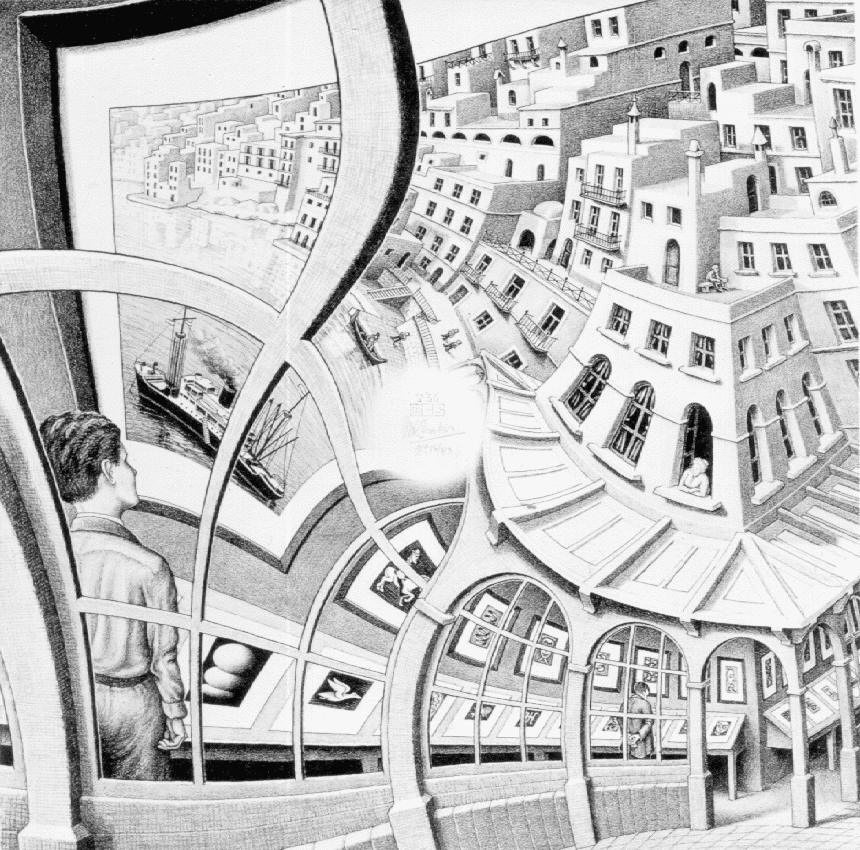
\includegraphics[width=0.5\columnwidth]{GalleriaStampe} 
% \caption[An example of a floating figure]{An example of a floating figure (a reproduction from the \emph{Gallery of prints}, M.~Escher,\index{Escher, M.~C.} from \url{http://www.mcescher.com/}).} % The text in the square bracket is the caption for the list of figures while the text in the curly brackets is the figure caption
% \label{fig:gallery} 
% \end{figure}

% \lipsum[10] % Dummy text

%------------------------------------------------

\subsection{Modelación del problema}

Representaremos los k compañeros de José como los vértices de un grafo no dirigido G = {V,E} de tamaño k, donde las relaciones de amistad entre ellos están representadas
por las aristas entre los vértices del grafo. Entonces analizaremos el problema de la siguiente forma :\\

Es posible eliminar aristas del grafo G (sin eliminarlas todas) de manera tal que todos los vértices queden, o bien aislados, o con exactamente 3 vecinos. \\

También podemos verlo de la siguiente manera: \\

Dado un grafo G determinar si existe un subgrago G' de G tal que G' es regular de grado 3.


\subsubsection{Np-Completitud}

Para demostrar que un problema es $NP-Completo$ hay que demostrar que:\\

1. El problema está en NP.

2. Se puede reducir un problema conocido como $NP-Completo$ a este problema en tiempo polinómico.

\textbf{Paso1: Probar que el problema de encontrar un subgrafo regular de grado 3 (SR3) está NP }\\


Dado un grafo G y un conjunto de aristas que supuestamente forman un subgrafo regular de grado 3, podemos verificar en 
tiempo polinomial si este subgrafo es regular de grafo 3. Para ello, recorremos todas las aristas del subgrafo y contamos el grado de
cada vértice. Si todos los vértices tienen grado 3, entonces el subgrafo es regular de grado 3. Este procedimiento tiene un costo de 
$O(|V|+|E|)$, siendo $|V|$ la cantidad de vértices y $|E|$ la cantidad de aristas.


\textbf{Paso2: Demostrar que SR3 es NP-Completo}\\

Para demostrar que el problema CSP es NP-completo, se necesita realizar una reducción desde un problema conocido como NP-completo. 
En este caso, se utilizará el problema de 3-coloración.


\textbf{ Problema de 3-coloración} \\


Dado un grafo no dirigido $G = (V,E)$ determinar si existe una partición del conjunto de vértices $V$,
def la forma ${V1,V2,V3}$ tal que no existen aristas entre los vertices que pertenecen a la misma partición $Vi$.\\


Definiciones:

- $G$ : Grafo de entrada del problema de 3-coloración.

- $V(G)$ : Conjunto de vértices del grafo $G$.

-$E(G)$ : Conjunto de aristas del grafo $G$. 

-$d(v_i)$ : Grado del vértice $i$.

-$K_n'$ :Grafo completo de n vértices al que se le quita una arista (este grafo tiene todos los vértices con grado n-1, excepto dos vértices que tienen grado n-2).

-3-partición : Dividir el conjunto de vértices en 3 conjuntos disjuntos.\\



\textbf{Paso3: Transformación de la entrada  }\\

A partir del grafo $G$, se construye un nuevo grafo $G'$ siguiendo los pasos siguientes:\\

1. \textbf{Ciclos} : Por cada vértice $v_i$ en $V(G)$, se crean 3 ciclos (denotados como : $C^1_i, C^2_i, C^3_i$), 
cada uno con una longitud de $2*d(v_i) + 1$. Los vértices de cada ciclo son denotados como $c^h_i_j$, $1 \leq i \leq n$,$ 1 \leq d \leq 2*d(v_i) + 1$,$ 1 \leq h \leq 3 $.\\

2. \textbf{Subgrafos} : Por cada arista $e_j \in E(G)$ se crean 3 subgrafos ($D^1_j, D^2_j, D^3_j$), donde cada uno es un $K_4'$. Los dos vértices con grado 2 en cada 
subgrafo son denotados como $x^h_i$ y $y^h_j$\\

3. \textbf{Conexiones} : Por cada arista entre los vértices $v_s$ y $v_t$ en G :

- Se seleccionan dos vértices $c^h_sa$ y $c^h_sb$ ($c^h_sa$ y $c^h_sb$) que aún tengan grado 2 de los ciclos correspondientes a $v_s$ y $v_t$, $C^h_s$ $(C^h_t)$.

- Por cada $1\leq h \leq 3$, se agregan a $G'$ las aristas $<c^h_sa,x^h_j>$, $c^h_ta,y^h_j$, $c^h_ta,x_h_j$ y $c^t_tb, y^h_j$\\

Una vez consideradas todas las aristas en
el paso (3), se tiene que para cada ciclo $C^h_i$ $( 1\leq i \leq n, 1 \leq h \leq 3 )$ solo queda un vértice con degree 2. Nombremos
dichos vértices como $w^h_i$.\\

4. \textbf{Construcción Adicional}: Por cada $1 leq i \leq n$, se construye un subgrafo $U_i$, que es un $K_4'$ más un vértice al que denominaremos $u_i$, los vértices de grado 2 del $K_4'$ los denominaremos 
$x_i$ y $y_i$, el vértice $u_i$ se une a los restantes del $K4'$ mediante una arista $<x_i, u_i>$. 

Se toman todos los grafos $U_i$ y se agregan a $G'$. junto con las aristas $<u_i,w^1_i>$, $<y_i, w^2_i>$ y $<y_i, w^3_i>$.\\


5. \textbf{Ciclo final} : Se agrega el ciclo $C'$ de longitud $2n$ a $G'$, conformado por los vértices ${a_11,..., a_1n, a21,..., a_2n}$ y se agregan las aristas $<a_pi, u_i>$ para $p = 1,2$.\\


\textbf{Paso4: Demostrar que G es 3-coloreable si y solo si G' tiene un subgrafo regular de grado 3  }\\

(\Rightarrow ) Sea G un grafo 3-coloreable, y una 3-partición de $V(G)$ tal que en cada conjunto $V_i$ queden solo vértices de un mismo color, entonces existe un grafo $H$, 
subgrafo inducido de $G'$ que es 3-regular, ya que siempre podemos tomar los vértices de la siguiente forma:

1. Todos los vértices $a_ij$ etán en $H$







\subsubsection{Solución}



%----------------------------------------------------------------------------------------
%	BIBLIOGRAPHY
%----------------------------------------------------------------------------------------

\renewcommand{\refname}{\spacedlowsmallcaps{References}} % For modifying the bibliography heading

\bibliographystyle{unsrt}

\bibliography{sample.bib} % The file containing the bibliography

%----------------------------------------------------------------------------------------

\end{document}